\documentclass{article}\usepackage[]{graphicx}\usepackage[]{color}
%% maxwidth is the original width if it is less than linewidth
%% otherwise use linewidth (to make sure the graphics do not exceed the margin)
\makeatletter
\def\maxwidth{ %
  \ifdim\Gin@nat@width>\linewidth
    \linewidth
  \else
    \Gin@nat@width
  \fi
}
\makeatother

\definecolor{fgcolor}{rgb}{0.345, 0.345, 0.345}
\newcommand{\hlnum}[1]{\textcolor[rgb]{0.686,0.059,0.569}{#1}}%
\newcommand{\hlstr}[1]{\textcolor[rgb]{0.192,0.494,0.8}{#1}}%
\newcommand{\hlcom}[1]{\textcolor[rgb]{0.678,0.584,0.686}{\textit{#1}}}%
\newcommand{\hlopt}[1]{\textcolor[rgb]{0,0,0}{#1}}%
\newcommand{\hlstd}[1]{\textcolor[rgb]{0.345,0.345,0.345}{#1}}%
\newcommand{\hlkwa}[1]{\textcolor[rgb]{0.161,0.373,0.58}{\textbf{#1}}}%
\newcommand{\hlkwb}[1]{\textcolor[rgb]{0.69,0.353,0.396}{#1}}%
\newcommand{\hlkwc}[1]{\textcolor[rgb]{0.333,0.667,0.333}{#1}}%
\newcommand{\hlkwd}[1]{\textcolor[rgb]{0.737,0.353,0.396}{\textbf{#1}}}%

\usepackage{framed}
\makeatletter
\newenvironment{kframe}{%
 \def\at@end@of@kframe{}%
 \ifinner\ifhmode%
  \def\at@end@of@kframe{\end{minipage}}%
  \begin{minipage}{\columnwidth}%
 \fi\fi%
 \def\FrameCommand##1{\hskip\@totalleftmargin \hskip-\fboxsep
 \colorbox{shadecolor}{##1}\hskip-\fboxsep
     % There is no \\@totalrightmargin, so:
     \hskip-\linewidth \hskip-\@totalleftmargin \hskip\columnwidth}%
 \MakeFramed {\advance\hsize-\width
   \@totalleftmargin\z@ \linewidth\hsize
   \@setminipage}}%
 {\par\unskip\endMakeFramed%
 \at@end@of@kframe}
\makeatother

\definecolor{shadecolor}{rgb}{.97, .97, .97}
\definecolor{messagecolor}{rgb}{0, 0, 0}
\definecolor{warningcolor}{rgb}{1, 0, 1}
\definecolor{errorcolor}{rgb}{1, 0, 0}
\newenvironment{knitrout}{}{} % an empty environment to be redefined in TeX

\usepackage{alltt}

\usepackage{amsmath}
\usepackage{amsthm}
\usepackage{amsfonts}

\title{Introduction to the Lab}
\author{Anh Le}
\IfFileExists{upquote.sty}{\usepackage{upquote}}{}
\begin{document}

\maketitle

\section{Class format}

\textbf{Before class}, you are expected the read the assigned sections from our textbooks. These are posted on the class website, under \textbf{``Meetings''}. I've chosen the sections that are most relevant to our work.

Read actively: 1) Type the code example into your own R while you read, 2) Test yourself by tweaking the input and guess the output.\\

\textbf{During class}, we won't waste everyone's time by lecturing and repeating the textbook. Instead, I will answer any question that you have and move on to exercises. Both of these are only beneficial if you have done the reading beforehand.

You guys will do these exercises at very different paces. So, if you are lucky to know some programming beforehand find these exercises easy, help your neighbors! I'll put up a Google doc on the projector so that anyone availble to help can put their names up.\\

\textbf{After class}, there will be exercises, mostly from the book and a few custom ones to familiarize you with Political Science data. These are posted on the class website, under \textbf{``Assignments''}. Homework submission and grading will be done through the website as well.\\

\begin{itemize}
\item Your homework will be graded by a randomly assigned classmate each week, based on solutions provided by me. This serves two purposes:
  \begin{enumerate}
    \item The long gap between submitting and receiving back homework often means that students do not look at the mistakes they make, defeating the purpose of doing exercise. Grading others' work keep the problem fresh in your mind.
    \item A programming puzzle can be solved in multiple ways, and thus it is very helpful to see other people's code. If your solution is more elegant than your peer's (or mine!), please show him/her by putting in comments when you grade.
\end{enumerate}
\item Do all of your homework using Rsweave, which allows you to embed R code directly within Latex. It takes minimal time to learn but will benefit hugely since you won't have to manually paste R code and figure into Latex. Like this:

\begin{knitrout}
\definecolor{shadecolor}{rgb}{0.969, 0.969, 0.969}\color{fgcolor}\begin{kframe}
\begin{alltt}
\hlnum{1} \hlopt{+} \hlnum{1}
\end{alltt}
\begin{verbatim}
## [1] 2
\end{verbatim}
\begin{alltt}
\hlkwd{plot}\hlstd{(}\hlkwd{rnorm}\hlstd{(}\hlnum{100}\hlstd{))}
\end{alltt}
\end{kframe}
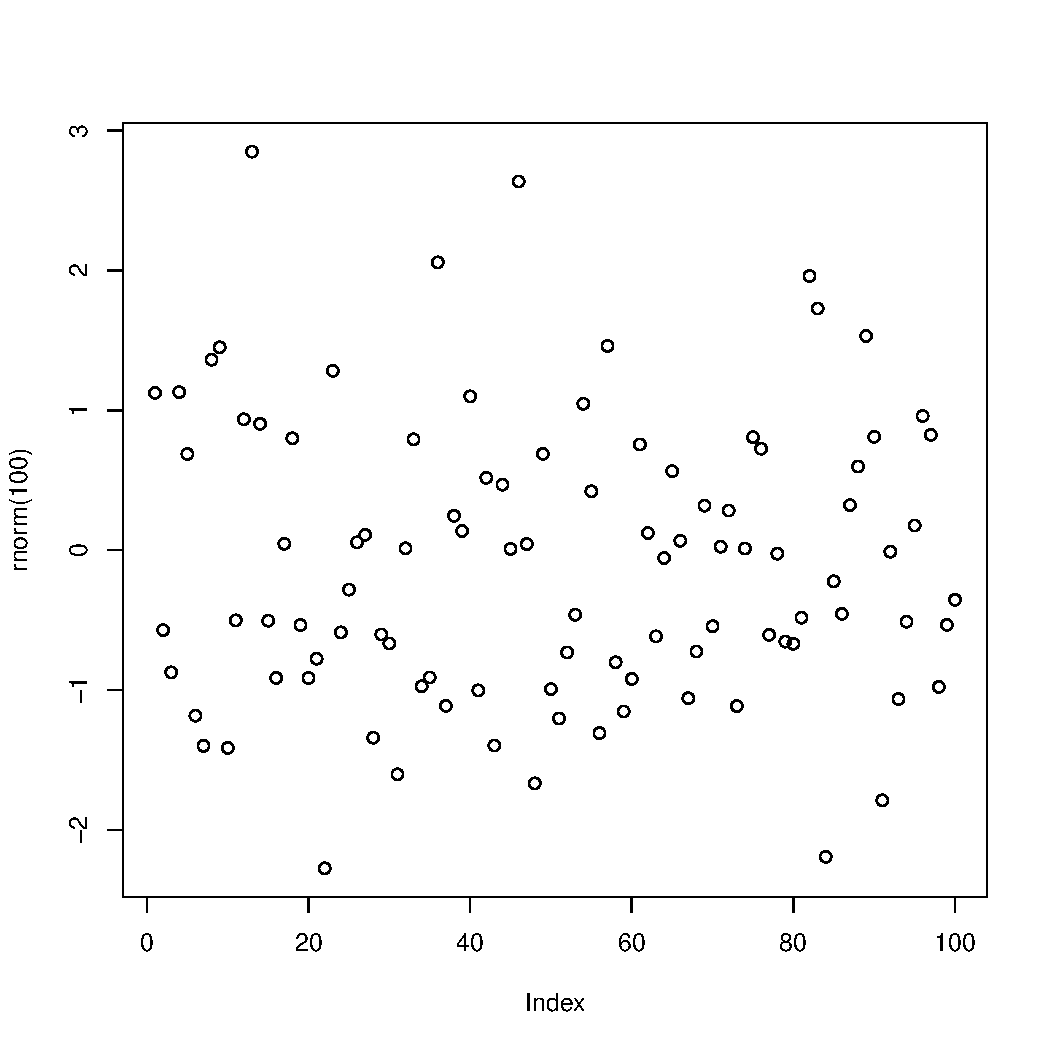
\includegraphics[width=\maxwidth]{figure/unnamed-chunk-1} 

\end{knitrout}

\item Everything you submit must be in two files: the .pdf and the source code (.Rnw). This also facilitates grading since the grader can directly edit the source code. {\color{red}Make sure to color your comment red}.

\item Late homework policy: The final grade of your assignment is calculated as following:
\[
\text{final grade} = \begin{cases}
      \text{raw grade} * 0.9^{\frac{n}{2}} & \text{if $n < 24$} \\
      0 & \text{if $n >= 24$}
    \end{cases}
\]
with $n$ being the number of hours late. In English, this means that for every two hour late, your grade decreases by 10\%. After 1 day late, the grade is automatically 0.
\end{itemize}

\section{How to get help}

This lab is only the very beginning of the your method training. Thus, it is important to learn to be self-sufficent. When you are stumped, do these things in order:

\begin{enumerate}
  \item Google it. It's a serious skill.
  \item Ask on the StackExchange network, i.e. Stackoverflow (stackoverflow.com) for programming question, and Crossvalidated (stats.stackexchange.com) for statistics question. There are thousands of helpful, active users on the site, so you can expect a well-formulated question to be answered in 20-30 minutes (which is much faster than emailing me). The site is such a wealth of knowledge that it is often the first result when you Google your question.

  Tips on StackExchange: People are much more willing to help if you show that you've done your research. Try to isolate the source of the error instead of posting your entire program. If people close your question because it's a duplicate or unclear, don't take it personal. Ask in the comment for reasons of closing, learn from the experience, and ask better question next time. StackExchange will be your best friend for the rest of your career, so get familiar with it now.

  \item If everything fails, ask me. Send me the link to the question you posted on StackExchange and I'll answer you there. Help you and help many others.
\end{enumerate}

\end{document}
